\begin{slikaDesno}{fig/Cload.pdf}
\PID
У колу напонског бафера са слике употребљен је
операциони појачавач са приближно једнополном фреквенцијском карактеристиком, у облику 
$A(\jj\upomega) = \dfrac{A_0}{1 + \jj\upomega/\upomega_0}$, $\upomega_0 = 2\uppi f_0$, $f_0 = 1\unit{Hz}$, $A_0 = 10^6$, а 
његова излазна отпорност износи $R_{\rm i} = 50\unit{\Omega}$. 
Израчунати максималну капацитивност $C_{\rm L}$, тако да је дато коло \textit{практично} стабилно.
\end{slikaDesno}

\REZULTAT


Коло је стабилно уколико је кружно појачање тамо где је фазно кашњење веће од $180{^\circ}$ мање од јединичног. Односно, уколико 
повратна спрега искључиво слаби фреквенцијске компоненте које могу довести до осциловања. 
Функција преноса кружног појачања $\upbeta A(s) = \dfrac{A_0}{1 + s/\upomega_0} \dfrac{1}{1 + s R_{\rm i} C_{\rm L}}$ је двополна,
са половима $-\upomega_0$ и $\upomega_{\rm p} = -1/{R_{\rm i}C_{\rm L}}$. На основу тога 
коло у строгом смислу никада не може бити нестабилно, јер фаза може бити закашњена за највише $180^\circ$. Међутим, у практичном смислу, уколико је појачање кола 
веће од 1 када се фазна карактеристика налази у околини кашњења од $180^\circ$, то значи да је систем изузетно осетљив на свако 
додатно кашњење које теоријски није узето у обзир, а које ће сигурно довести до осцилација кола. Из тог разлога, као добру 
процену границе практичне стабилности, можемо наметнути да појачање буде мање од 1 онда када 
апроксимативна Бодеова карактесристика достигне кашњење од 
$180^\circ$. Критични случај је приказан на слици \ref{fig:\ID:grafik}, једну декаду
касније у односу на пол који умеће филтар који чине кондензатор $C_{\rm L}$ и излазна отпорност ОП.
 
%
\noindent
\begin{minipage}[t]{0.45\textwidth}
    \vspace{-0pt}
    \centering
    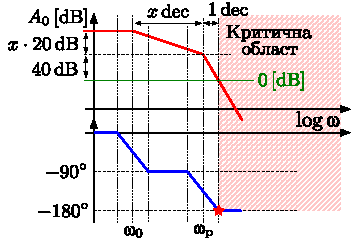
\includegraphics[scale=1]{fig/Cload_grafik.pdf}
    \captionof{figure}{апроксимативне Бодеове карактеристике, амплитудска и фазна.}
    \label{fig:\ID:grafik}
\end{minipage}
%
\begin{minipage}[t]{0.55\textwidth}
Са слике се има да је критични 
учестаност када фазна карактеристика достиже вредност кашњења од $180^\circ$, тачно једну декаду касније од 
пола $\upomega_{\rm p}$, што за последицу има да амплтитуда појачања на месту тог пола треба да буде тачно $40\unit{dB}$.
Број декада $x$ између полова $\upomega_{\rm p}$ и $\upomega_{0}$, под нагибом од $20\unit{dB/dec}$ треба да 
доведе до појачања ОП на ниским учестаностима, односно $A_0\unit{[dB]} = 20\log_{10}(A_0) = 120\unit{dB}$. На основу тога 
поставља се једнакост
\begin{equation}
        40\unit{dB} + 20x \unit{dB} = 120\unit{dB}
\end{equation}
Чије је решење $x = 4$, па закључујемо да је $\upomega_{\rm p } = 10^4 \upomega_{0} $.
\end{minipage}
На основу тога, одређује се критична вредност капацитивности 
$C_{\rm L} = \dfrac{1}{\upomega_{\rm p} R_{\rm i}} \approx 320\unit{nF}$. 